\subsubsection{NASA-TLX}
\label{subsubsec:results_nasa_tlx_1}

The NASA-TLX provides two information that are relevant to the workload analysis. The first one is the score attributed to the ‘mental demand’ dimension. The second one is the average obtained from the scores of the six dimensions of NASA-TLX. The two analyses are presented in the next subsections.

\paragraph{Analysis of the mental demand scale}\mbox{}\\

Table \ref{tab:md_table_blind} presents the ‘mental demand’ score attributed by each blind participant to each guidance method. The ‘base’ method refers to the guidance method that the person uses in his/her daily life (e.g., white cane). 


\begin{table}[!htb]
\centering
\caption{Score of NASA-TLX mental demand for the blind participants.}
\label{tab:md_table_blind}
\begin{tabular}{llrrrrr}
\toprule
     &        & Base & Audio & \begin{tabular}[c]{@{}l@{}}Haptic\\ Belt\end{tabular} & \begin{tabular}[c]{@{}l@{}}Virtual\\ Cane\end{tabular} & Mixture \\
Participant & Round &      &       &                                                       &                                                        &         \\
\midrule
001C & First &    3 &     1 &                                                    14 &                                                      3 &       6 \\
     & Return &    1 &     1 &                                                    10 &                                                      2 &       6 \\
002C & First &    5 &     1 &                                                     1 &                                                     10 &      12 \\
     & Return &    1 &     1 &                                                     1 &                                                     10 &       3 \\
003C & First &    5 &     5 &                                                     5 &                                                      8 &       1 \\
     & Return &    3 &     1 &                                                     1 &                                                      2 &       1 \\
004C & First &    9 &    10 &                                                    15 &                                                     10 &      10 \\
     & Return &    7 &    10 &                                                    14 &                                                      8 &      10 \\
\bottomrule
\end{tabular}
\end{table}



The mean value obtained for each guidance method is illustrated in Figure \ref{fig:barplot_md_avg_5_scene_blind}. It shows a systematic reduction on the perceived mental workload between the rounds for all methods, confirming that the participants get familiar with the devices after the first use. It also shows that although the haptic belt obtained the largest mean, it also had the largest variation, showing that the effort required from the user may vary significantly.

\begin{figure}[!htb]
    \centering
    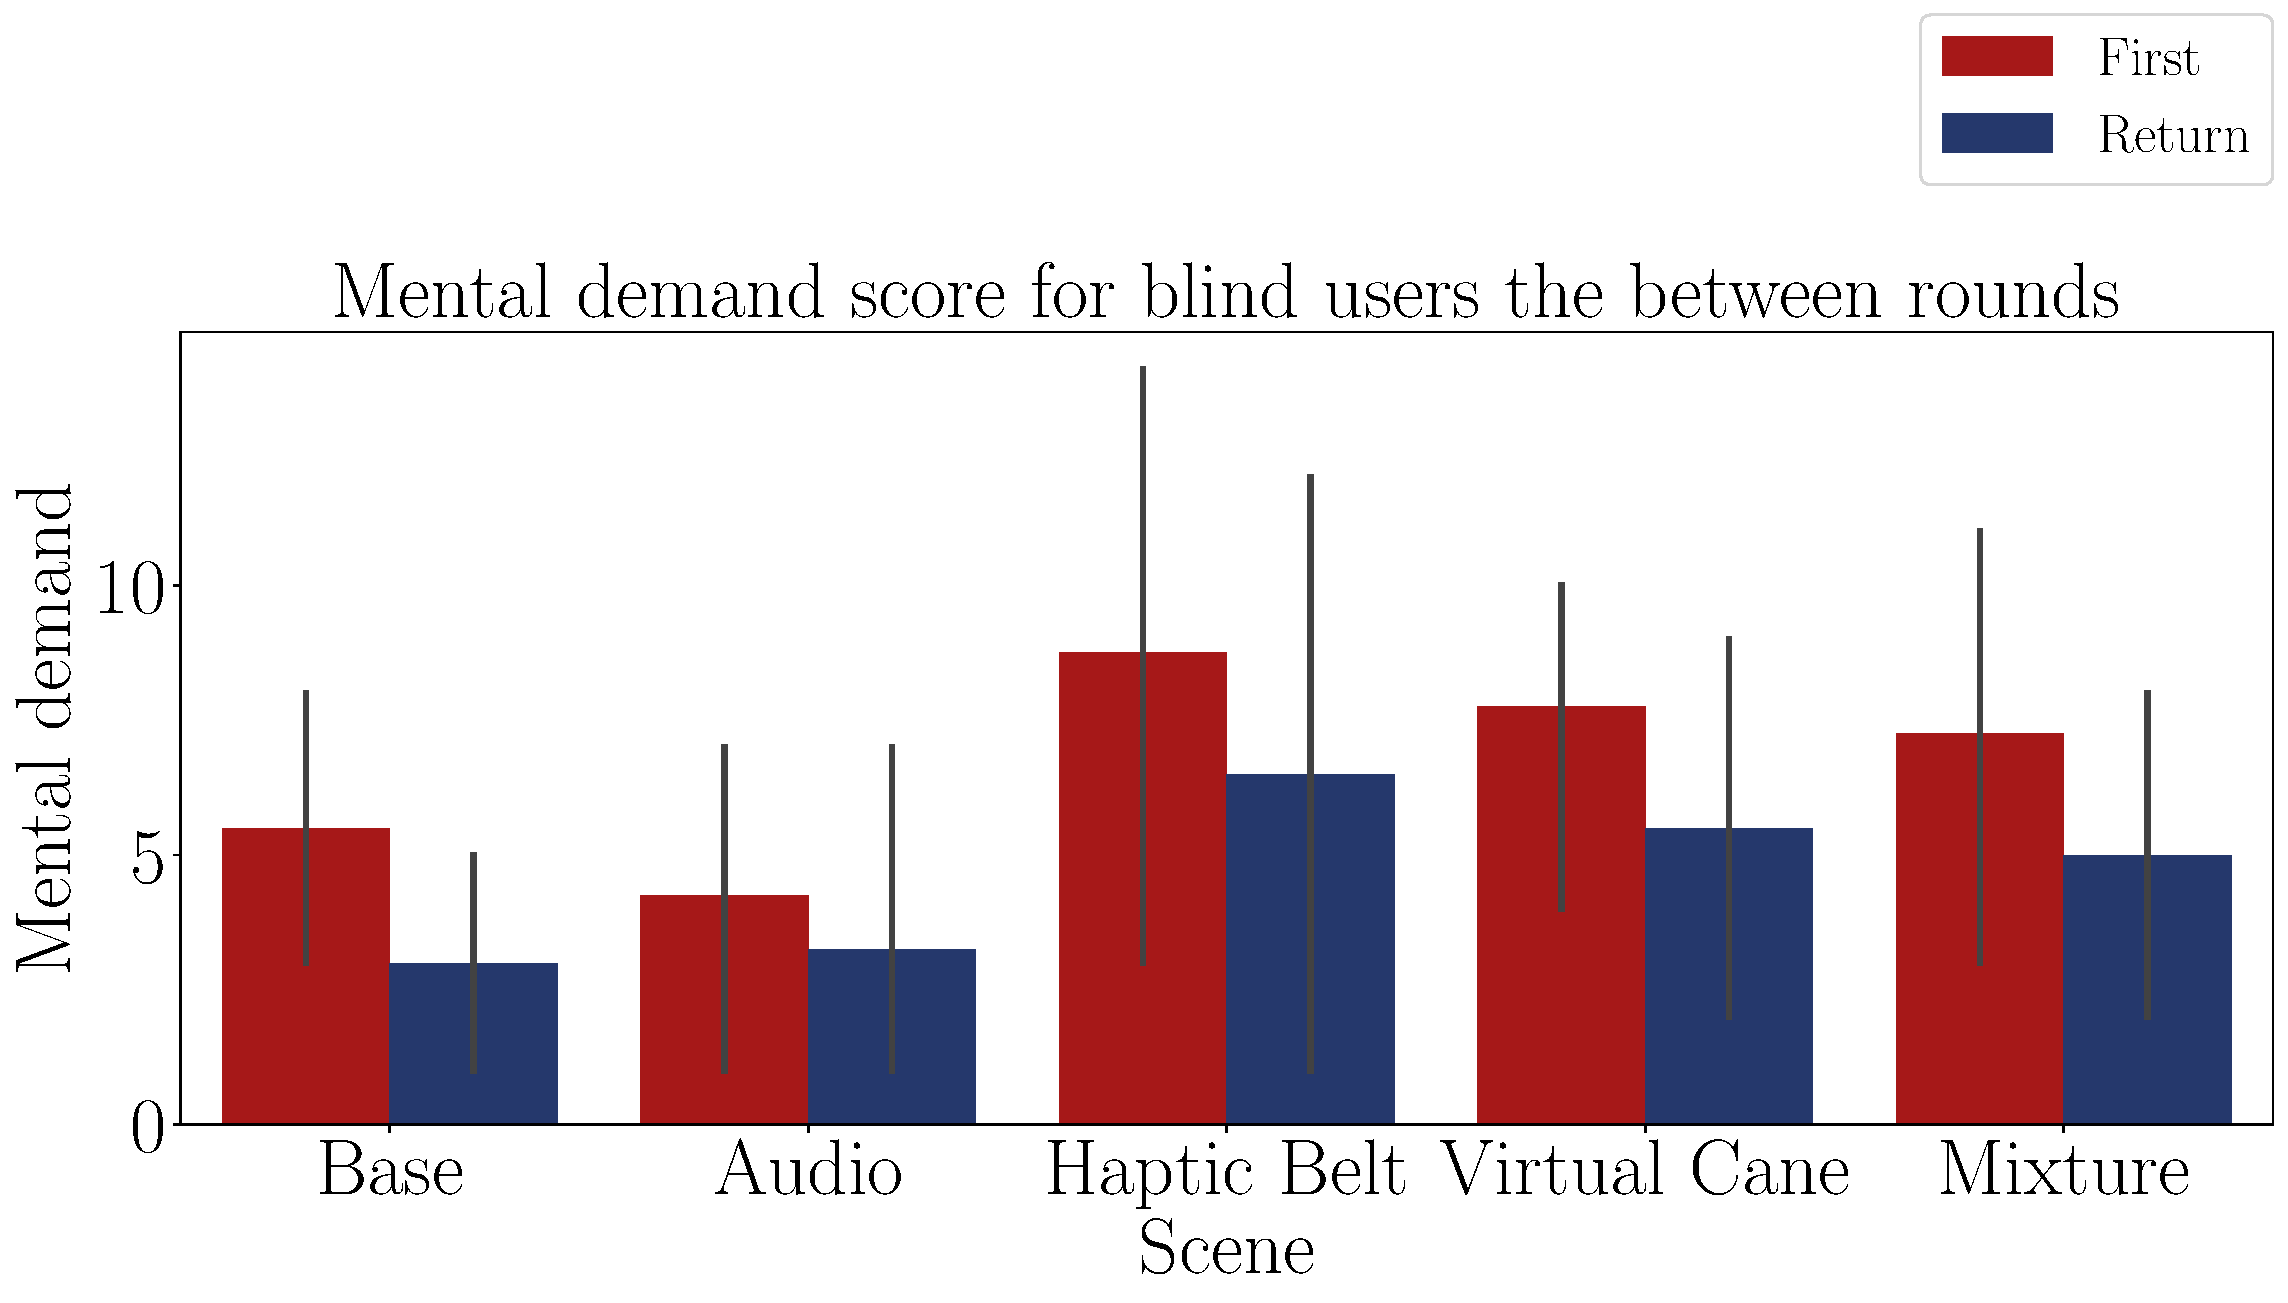
\includegraphics[width = \textwidth]{Resultados/Nasa/Figuras/pdf/barplot_md_avg_5_scene_blind.pdf}
    \caption{Mean and standard deviation of mental demand of blind participants for each method.}
    \label{fig:barplot_md_avg_5_scene_blind}
\end{figure}


Figure \ref{fig:boxplot_md_blind_scene}  presents a box plot of the mental demand score grouped by method. This Figure shows that there may be two different groups: one associated with lower demand, composed of ‘base’ and ‘audio’, and another with higher demand, composed of ‘haptic belt’, ‘virtual cane’ and ‘mixture’. It indicates that maybe a guidance method that uses vibration as input is not intuitive. Following, Figure \ref{fig:boxplot_md_blind_rounds} presents a box plot of the mental demand grouped by the rounds, confirming the general tendency to reduce the required ‘mental demand’. 

\begin{figure}[!htb]
    \centering
    \begin{minipage}{0.45\textwidth}
        \centering
        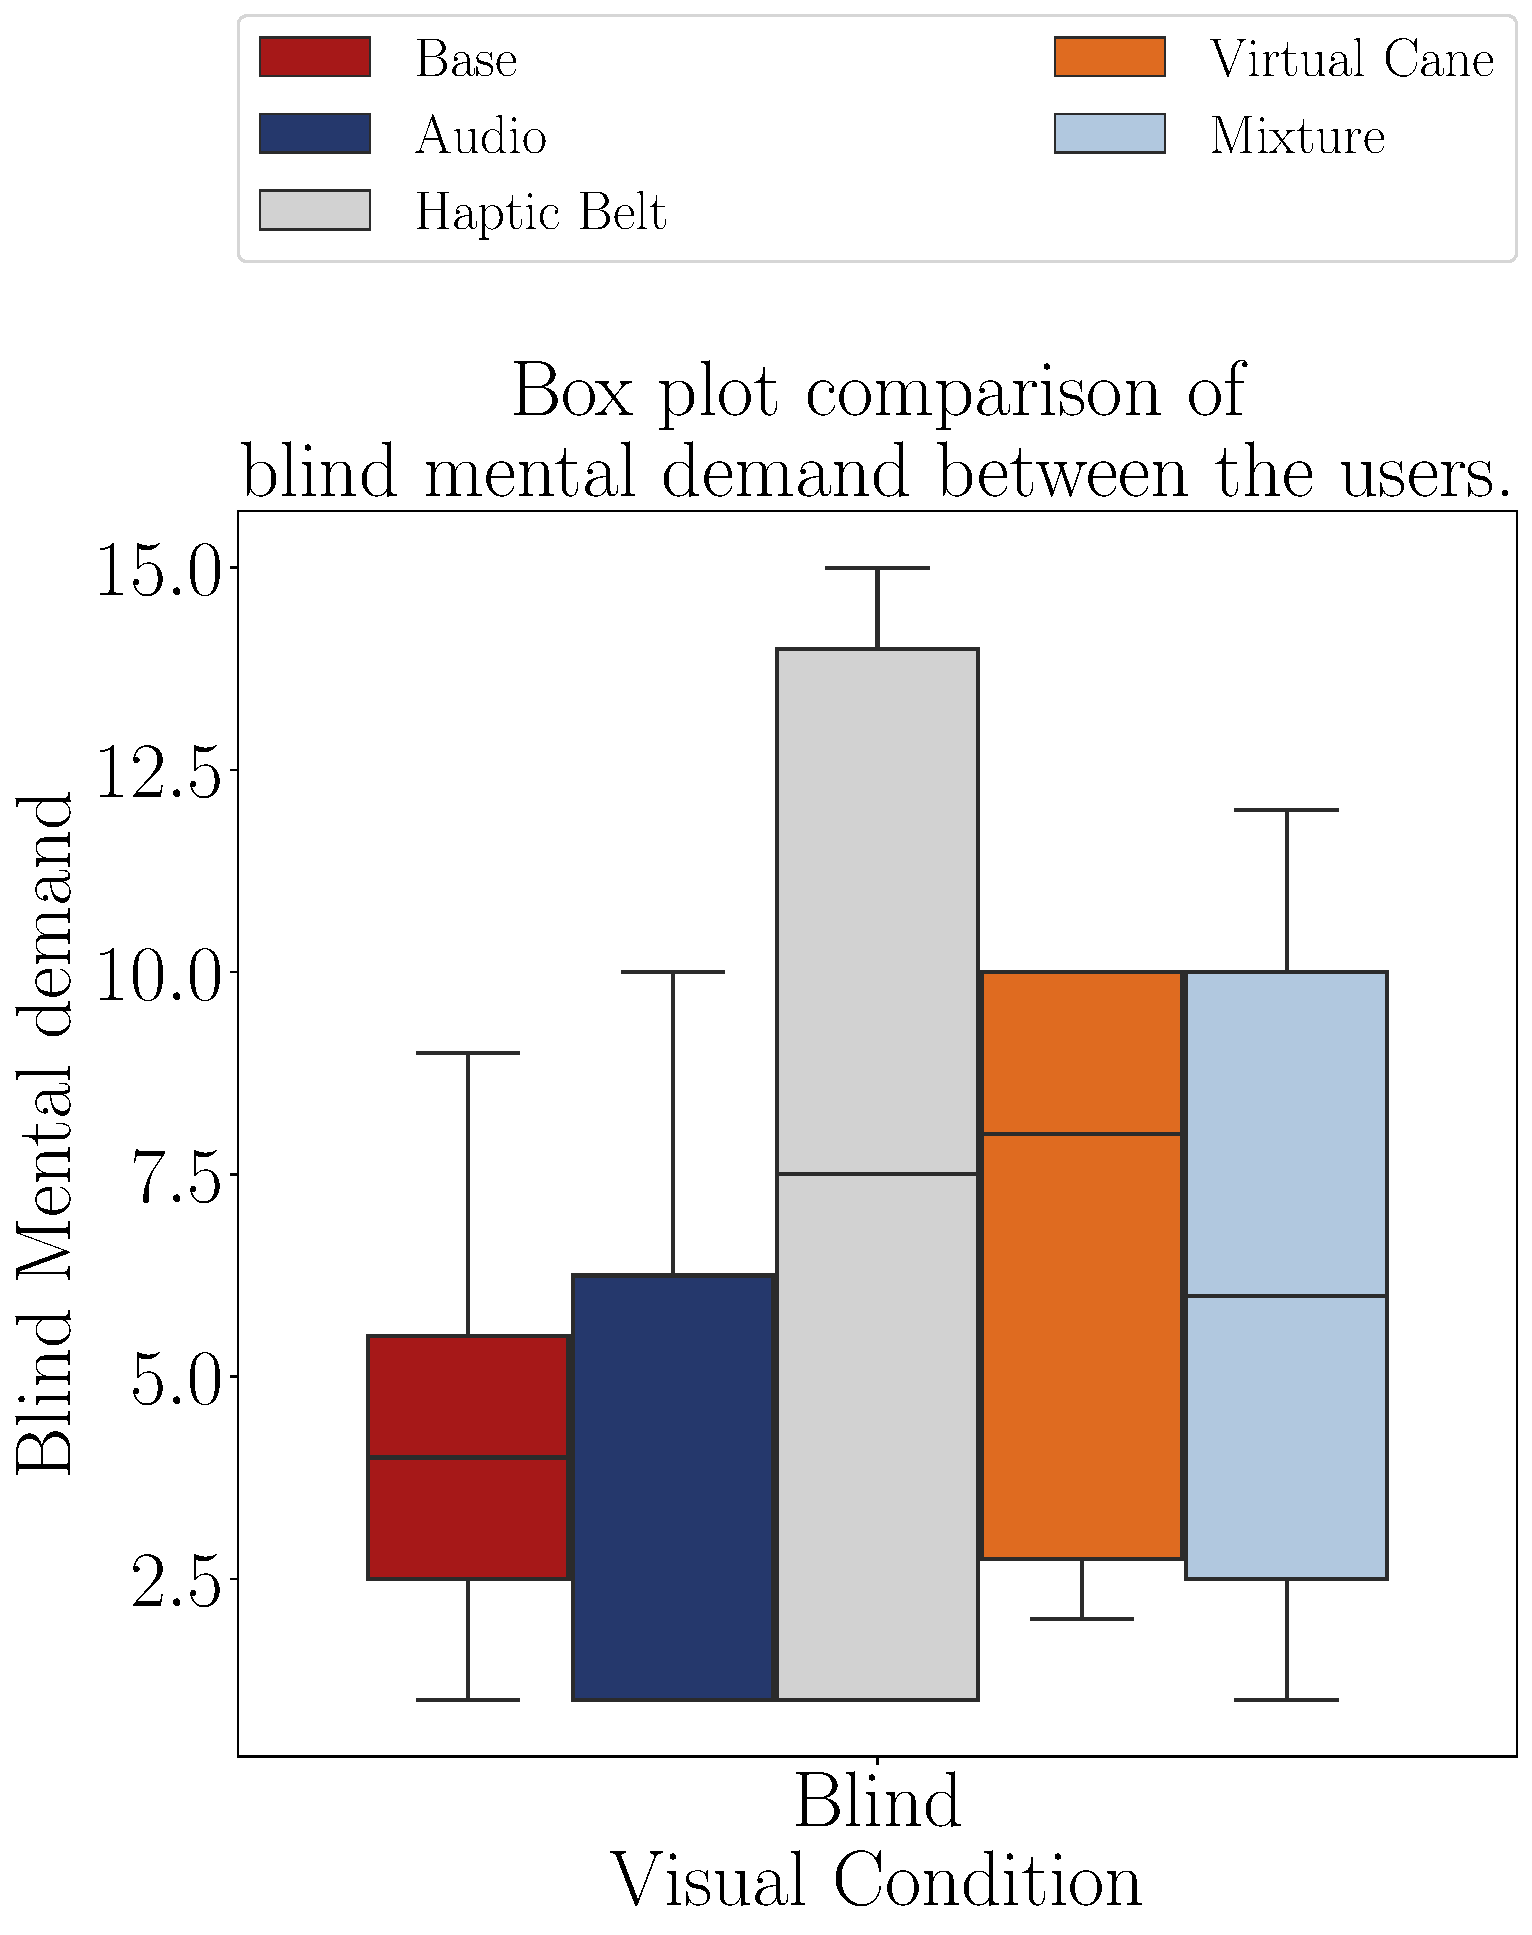
\includegraphics[width = \textwidth]{Resultados/Nasa/Figuras/pdf/boxplot_md_blind_scene.pdf}
        \caption{Boxplot of the mental demand of the blind participants grouped by method.}
        \label{fig:boxplot_md_blind_scene}
    \end{minipage}
    \begin{minipage}{0.075\textwidth}
        \hfill
    \end{minipage}
    \begin{minipage}{0.45\textwidth}
        \centering
        %\vspace{3ex}
        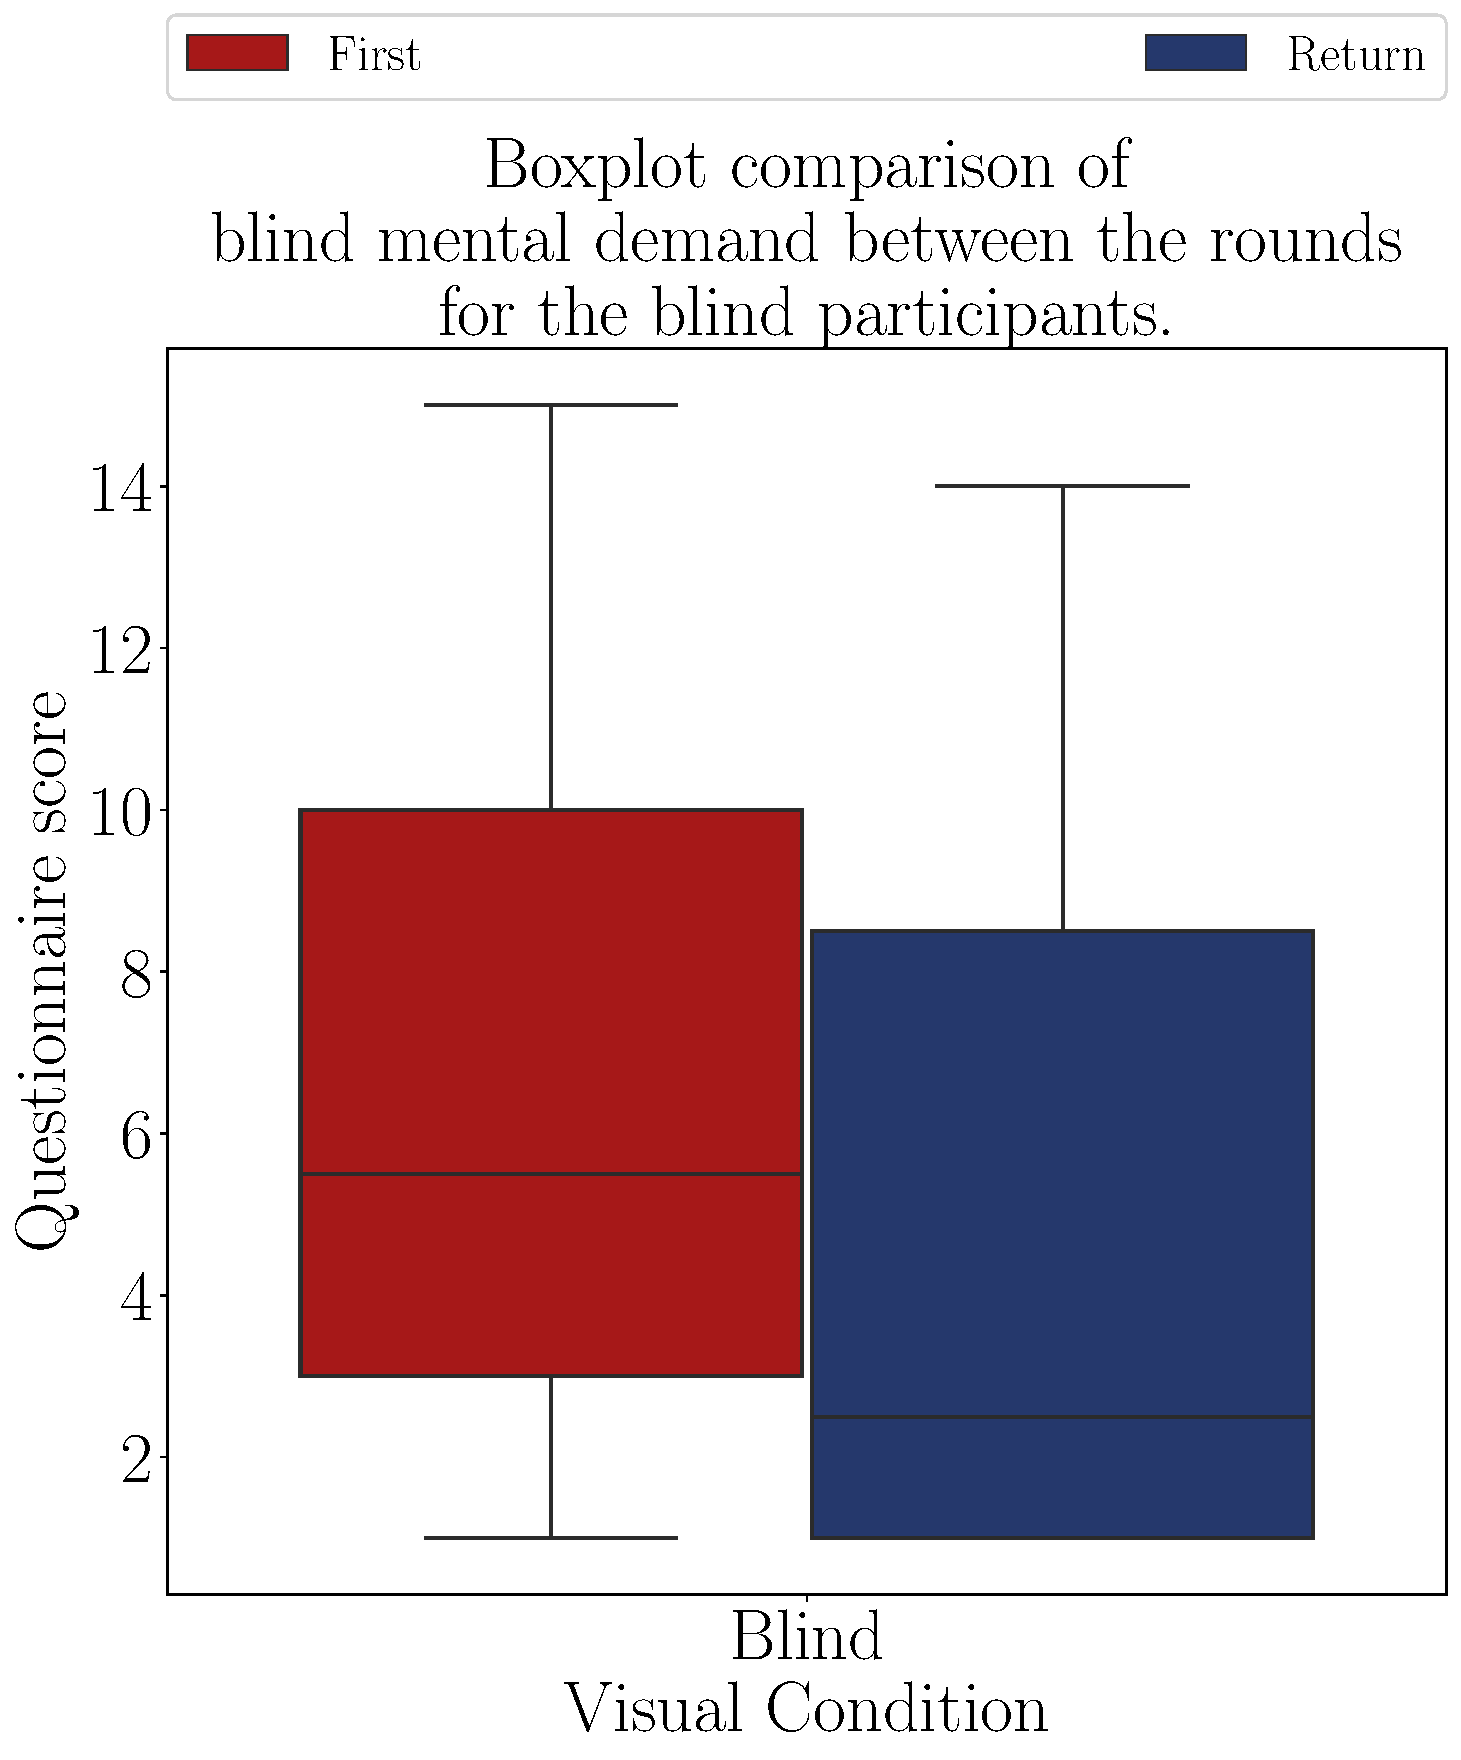
\includegraphics[width = \textwidth]{Resultados/Nasa/Figuras/pdf/boxplot_md_blind_rounds.pdf}
        \caption{Boxplot of the mental demand of the blind participants grouped by round.}
        \label{fig:boxplot_md_blind_rounds}
    \end{minipage}
\end{figure}

In order to support the statistical analysis, Figures \ref{fig:qqplot_md_avg_two_way_blind} and \ref{fig:residplot_md_avg_two_way_blind} presents the QQ-plot and the residual plot of the ‘mental demand’ data, confirming that the data follow a normal distribution and the residues are homogenous.

Following, Figures \ref{fig:qqplot_md_avg_two_way_blind} and \ref{fig:residplot_md_avg_two_way_blind} shows the distribution and variance of the Table \ref{tab:md_table_blind}. These Figures shows that the data are normally distributed and that the methods have a similar variance. The Table \ref{tab:blocanova_md_avg_two_way_blind} shows the Anova test p-values of the mental demand of the ‘blind” sample between the guidance methods. The method’s and the round’s p-values indicates that there is no influence from them in the mental demand. The interaction between the methods and the round also does not influences the mental demand.

\begin{figure}[!htb]
    \centering
    \begin{minipage}{0.45\textwidth}
        \centering
        %\vspace{1ex}
        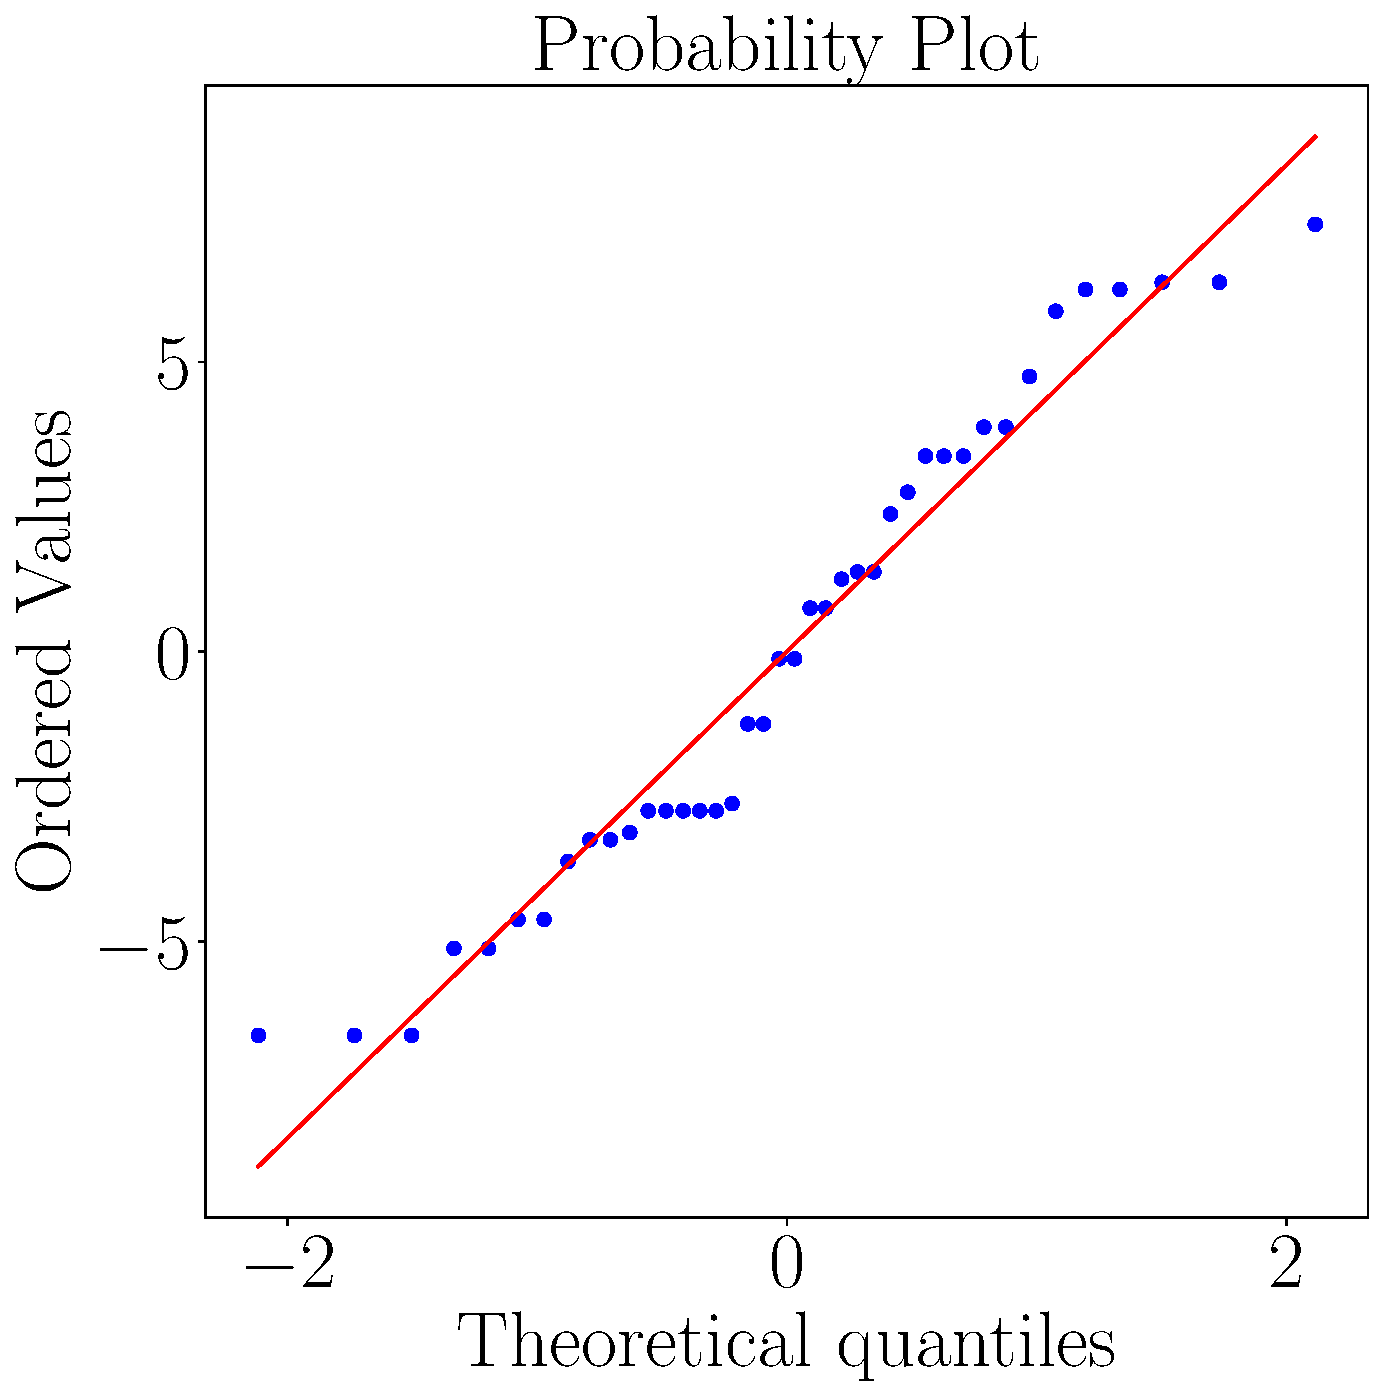
\includegraphics[width = \textwidth]{Resultados/Nasa/Figuras/pdf/qqplot_md_avg_two_way_blind.pdf}
        \caption{QQ plot of the mental demand of the blind participants on each method.}
        \label{fig:qqplot_md_avg_two_way_blind}
    \end{minipage}
    \begin{minipage}{0.075\textwidth}
        \hfill
    \end{minipage}
    \begin{minipage}{0.45\textwidth}
        \centering
        %\vspace{1ex}
        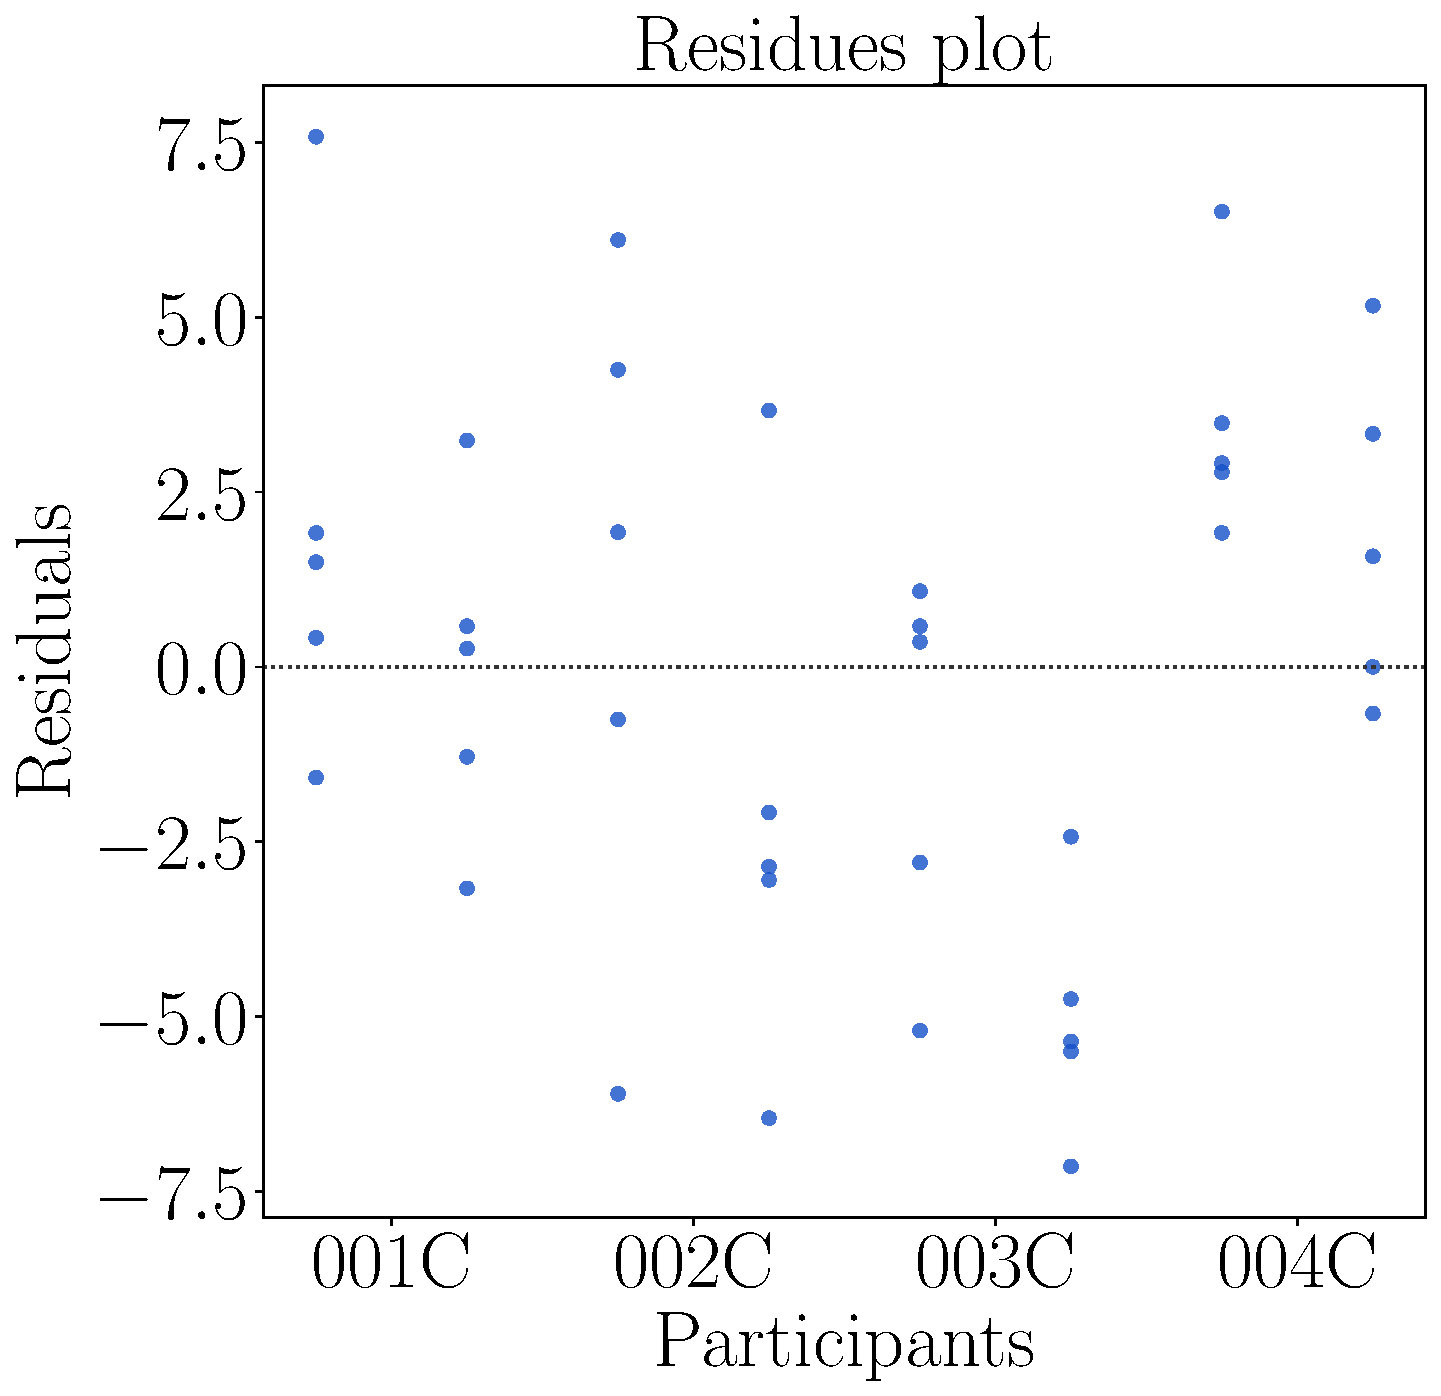
\includegraphics[width = \textwidth]{Resultados/Nasa/Figuras/pdf/residplot_md_avg_two_way_blind.pdf}
        \caption{Residual plot of the mental demand score the blind participants on each method.}
        \label{fig:residplot_md_avg_two_way_blind}
    \end{minipage}
\end{figure}

Following, the statistical model of Equation 5.1 is used for the analysis of variance (ANOVA): 

\begin{equation}
    \label{eq:statistical_model}
    y_{ijk} = \mu + \tau_i + \beta_j + \msout{\omega_k} + (\tau\beta_{ij}) + e
\end{equation}

where:

\begin{itemize}
    \item $y_{ij}$ - output variable for method $i$, round $j$ and participant $k$;
    \item $\mu$ - mean of all the observations;
    \item $\tau_i$ - variance from method $i$;
    \item $\beta_j$ - variance from round $j$;
    \item \sout{$\omega_k$} - variance from participant k, which is treated as a block;
    \item $\tau\beta_{ij}$ - combined variance from the interaction between method i and round j;
    \item $e$ - residual error.
\end{itemize}

The results of ANOVA are presented in Table \ref{tab:blocanova_md_avg_two_way_blind}. ANOVA tests the hypothesis that the means of independent groups of data are equal or not. In the literature, a p-value of 0.05 is commonly adopted as a threshold to confirm the hypothesis. A p-value < 0.05 indicates that the means of the groups are statistically different with 95\% of confidence. According to this criterion neither method or round have a significant influence on the mental demand.

However, due to the low number of participants, the threshold of 0.1 could also be considered. In this case, it indicates, with 90\% confidence, that the mean of the ‘first’ and ‘return’ rounds are different. For guidance method, the p-value of 0.170 is close to the threshold but slightly higher, suggesting that the means may be different but this hypothesis is not statistically confirmed with the current data. 


\begin{table}[!htb]
\centering
\caption{Anova p-value for the mental demand average on each method for blinded users.}
\label{tab:blocanova_md_avg_two_way_blind}
\begin{tabular}{lrrrrl}
\toprule
               Source &  Squared sum &  DOF & Squared average &     F & \begin{tabular}[c]{@{}l@{}}P-Value \\ $(F_{0} > F)$\end{tabular} \\
\midrule
Participants (Blocks) &      298.475 &    3 &          99.492 & 8.133 &                                                                  \\
         \    Methods &       85.150 &    4 &          21.288 & 1.740 &                                                            0.170 \\
          \    Rounds &       42.025 &    1 &          42.025 & 3.436 &                                                            0.075 \\
     \    Interaction &        2.850 &    4 &           0.712 & 0.058 &                                                            0.993 \\
   Experimental Error &      330.275 &   27 &          12.232 &       &                                                                  \\
                Total &      758.775 &   39 &                 &       &                                                                  \\
\bottomrule
\end{tabular}
\end{table}



In order to conclude the analysis of the NASA-TLX mental demand, Table \ref{tab:md_var_average_group_blind} brings the average of difference between the mental demand of the ‘first’ and ‘return’ rounds. Unexpectedly, it shows that the largest variation is obtained to the ‘base’, i.e., the guidance method the participant is used to and, therefore, should not present a significant variation. The method with the lower variation was ‘audio’, probably because it already had a very low score in the first round. 


\begin{table}[!htb]
\centering
\caption{Mental demand variation grouped by participant and visual condition}
\label{tab:md_var_average_group_blind}
\begin{tabular}{lrrrrrr}
\toprule
{} &  Base & Audio & \begin{tabular}[c]{@{}l@{}}Haptic\\ Belt\end{tabular} & \begin{tabular}[c]{@{}l@{}}Virtual\\ Cane\end{tabular} & Mixture \\
Visual Condition &       &       &                                                       &                                                        &         \\
\midrule
Blind            &  -2.5 &  -1.0 &                                                  -2.2 &                                                   -2.2 &    -2.2 \\
\bottomrule
\end{tabular}
\end{table}



\FloatBarrier

%%%%%%%%%%%%%%%%%%%%%%%%%%%%%%%%%%%%%%%%%%%%%%%%%%%%%%%%%%%%%%%%%%%%%%%%%%%
%%%%%%%%%%%%%%%%%%%%%%%%%%%%%%%%%%%%%%%%%%%%%%%%%%%%%%%%%%%%%%%%%%%%%%%%%%%
%%%%%%%%%%%%%%%%%%%%%%%%%%%%%%%%%%%%%%%%%%%%%%%%%%%%%%%%%%%%%%%%%%%%%%%%%%%
%%%%%%%%%%%%%%%%%%%%%%%%%%%%%%%%%%%%%%%%%%%%%%%%%%%%%%%%%%%%%%%%%%%%%%%%%%%


\paragraph{Analysis of the NASA-TLX score}\mbox{}\\

This section repeats the analysis steps of the previous section but now considering the mean value of all dimension of NASA-TLX, referred in this text as global score. Table \ref{tab:nasa_table_blind} presents the global score of each blind participant. 


\begin{table}[!htb]
\centering
\caption{NASA-TLX score felled by the blinded participants.}
\label{tab:nasa_table_blind}
\begin{tabular}{llrrrrr}
\toprule
     &        &  Base &  Audio & \begin{tabular}[c]{@{}l@{}}Haptic\\ Belt\end{tabular} & \begin{tabular}[c]{@{}l@{}}Virtual\\ Cane\end{tabular} & Mixture \\
Participant & Round &       &        &                                                       &                                                        &         \\
\midrule
001C & First & 4.833 &  4.000 &                                                 8.833 &                                                  5.167 &   6.333 \\
     & Return & 4.167 &  4.000 &                                                 6.667 &                                                  4.500 &   6.167 \\
002C & First & 6.333 &  4.833 &                                                 4.833 &                                                  9.000 &   7.000 \\
     & Return & 4.500 &  4.833 &                                                 4.833 &                                                  7.000 &   5.167 \\
003C & First & 4.000 &  4.000 &                                                 5.333 &                                                  6.667 &   3.500 \\
     & Return & 4.000 &  3.833 &                                                 3.667 &                                                  3.500 &   3.500 \\
004C & First & 9.833 & 10.000 &                                                12.667 &                                                  9.667 &  11.000 \\
     & Return & 8.667 &  9.167 &                                                11.667 &                                                  9.333 &  10.833 \\
\bottomrule
\end{tabular}
\end{table}



Figure \ref{fig:barplot_nasa_avg_5_scene_blind} brings the corresponding barplot with the mean value and standard deviation for each guidance method and each round. In a qualitative comparison with Figure \ref{fig:barplot_md_avg_5_scene_blind}, the differences between the methods are confirmed but softened. It is possible to notice that the mean score of ‘audio’ and ‘base’ are still lower than that of the other methods. The differences between ‘first’ and ‘return’ rounds are also reduced. However, the standard deviation among are also considerably reduced for all methods, and especially for the haptic belt.

\begin{figure}[!htb]
    \centering
    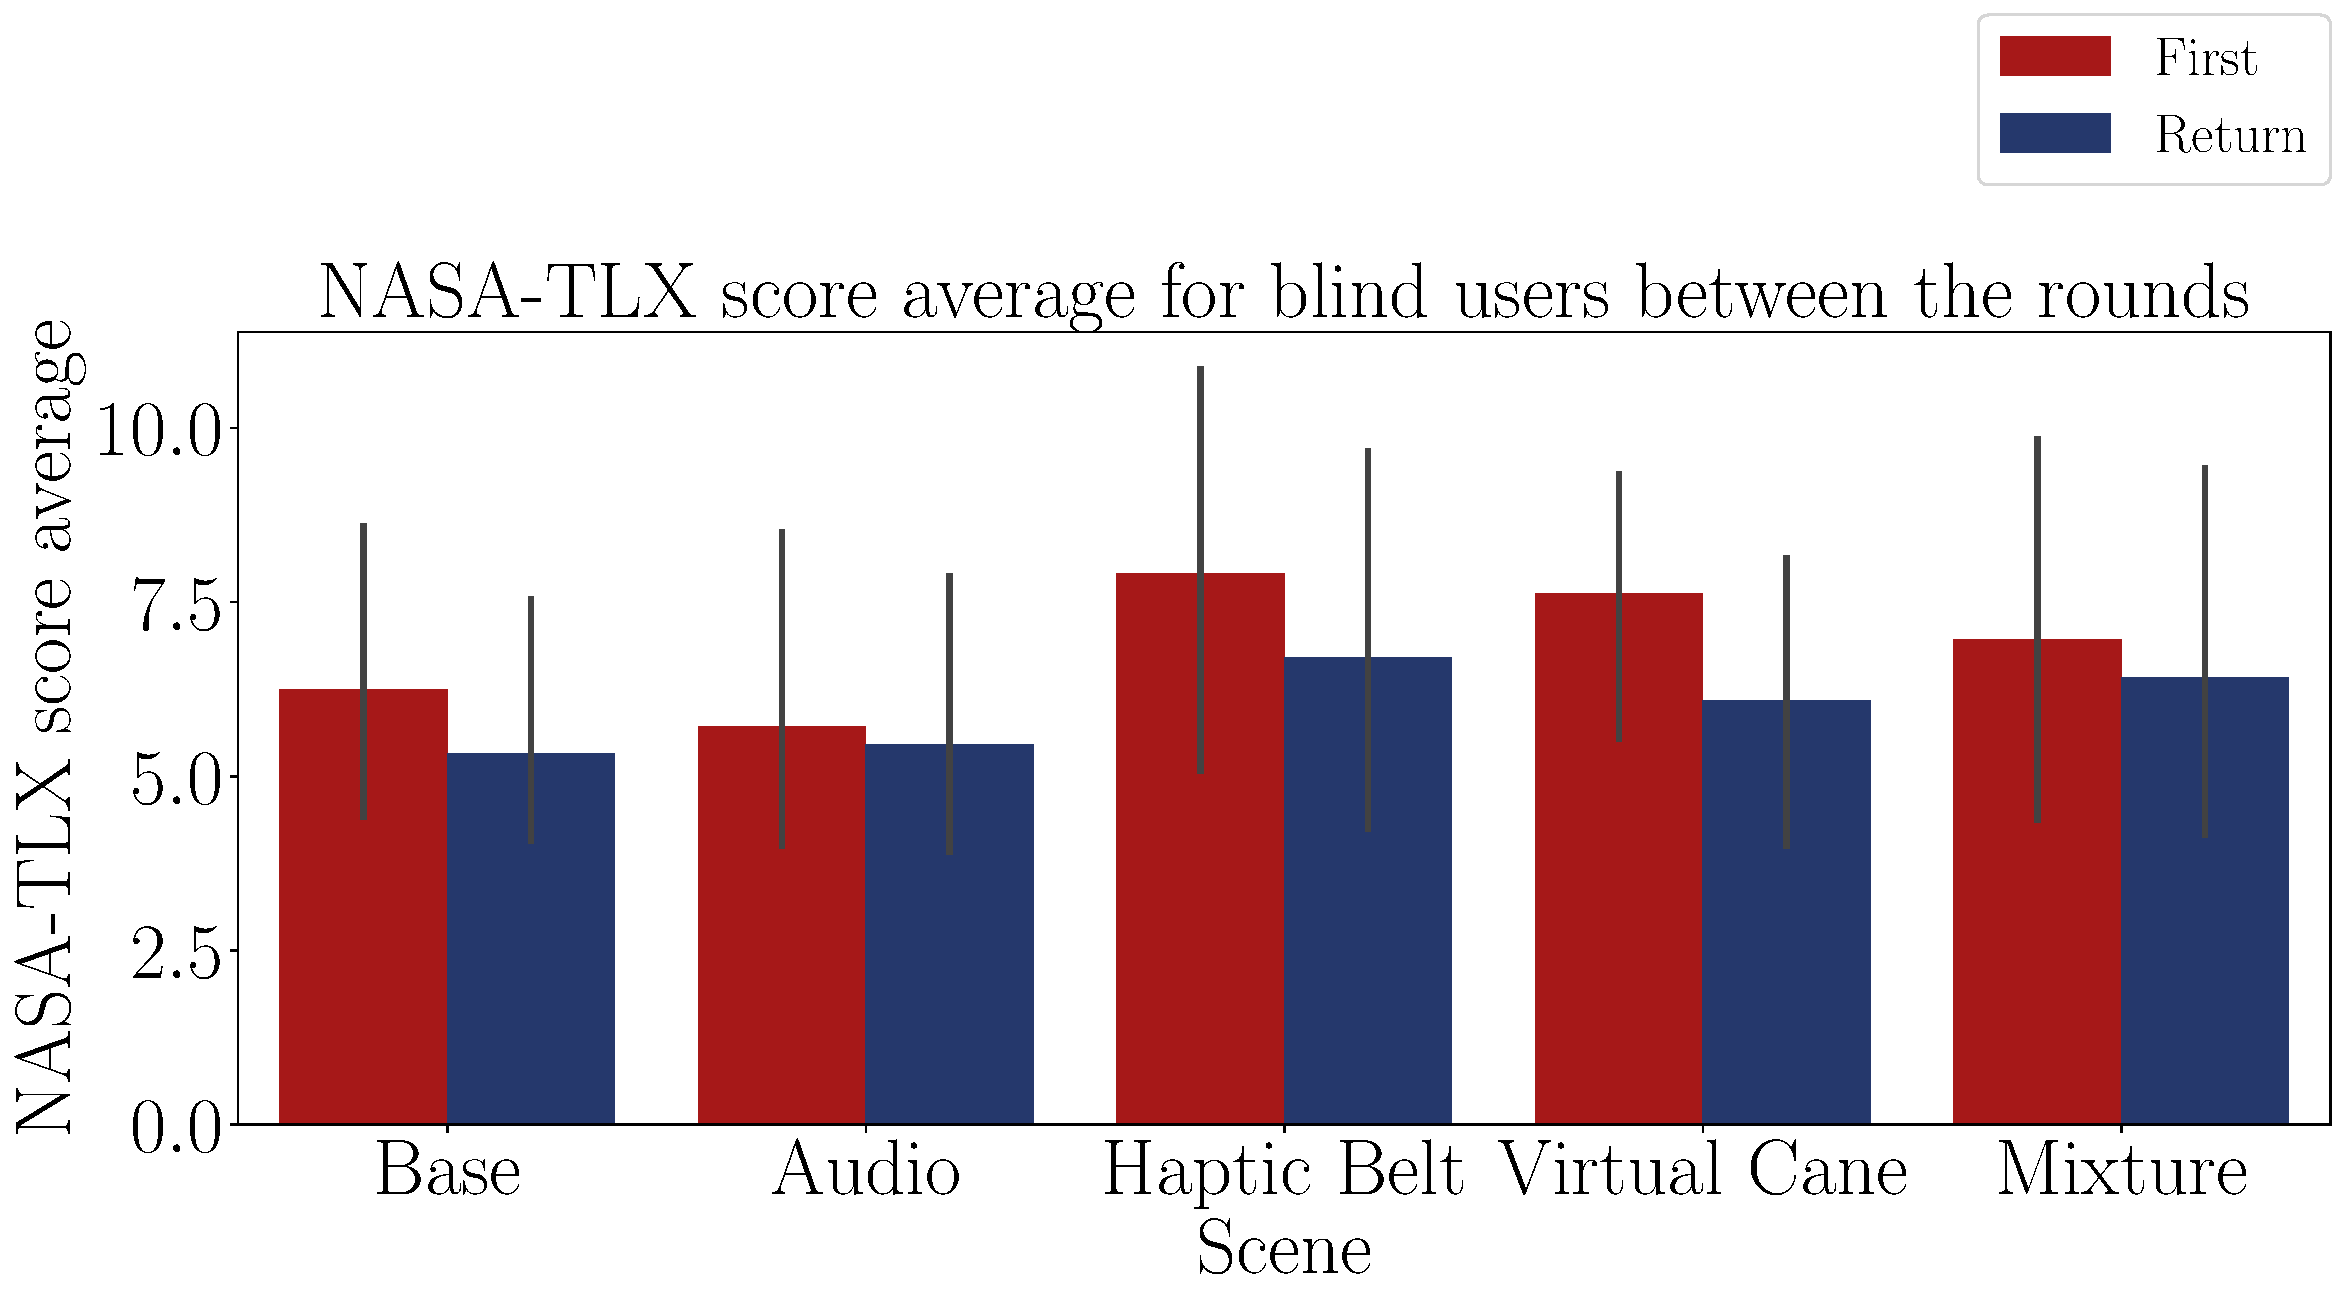
\includegraphics[width = \textwidth]{Resultados/Nasa/Figuras/pdf/barplot_nasa_avg_5_scene_blind.pdf}
    \caption{Barplot of the average NASA-TLX score of the blind participants on each method.}
    \label{fig:barplot_nasa_avg_5_scene_blind}
\end{figure}

Figure \ref{fig:boxplot_nasa_blind_scene} presents the box plot with the NASA-TLX global score grouped by method. Similar to what happened for the ‘mental demand’, it shows that it possible to split the methods in two different groups: ’base’ and ‘audio’, which requires a lower level of workload, and another group, which requires a higher level. Figure \ref{fig:boxplot_nasa_blind_rounds} presents a box plot with the NASA-TLX global score grouped by the rounds, apparently showing that the two groups are still different. 

\begin{figure}[!htb]
    \centering
    \begin{minipage}{0.45\textwidth}
        \centering
        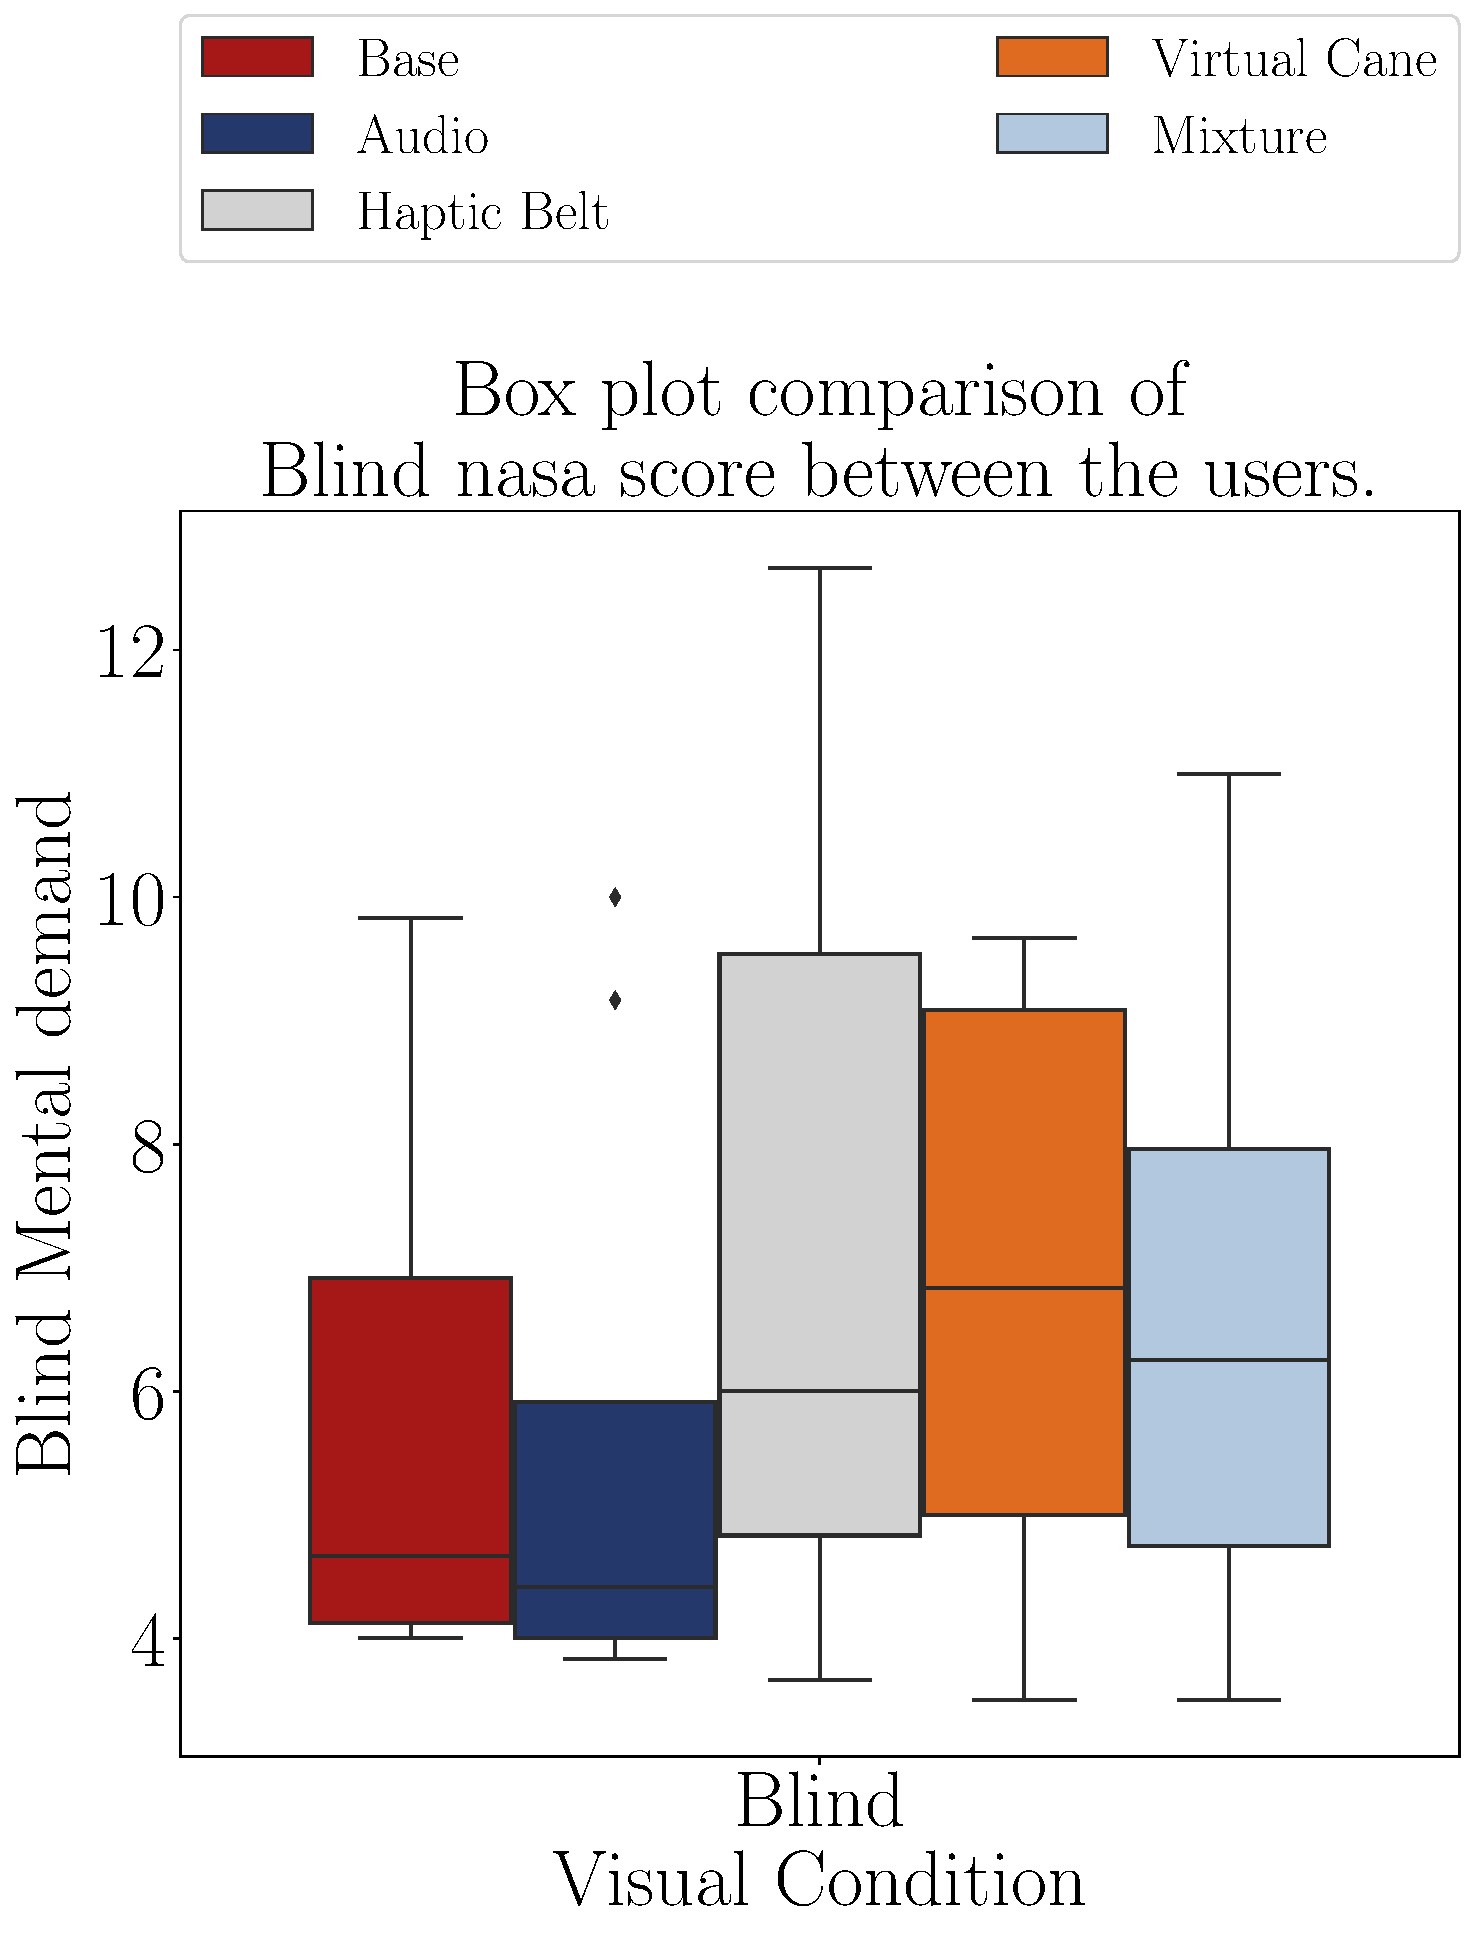
\includegraphics[width = \textwidth]{Resultados/Nasa/Figuras/pdf/boxplot_nasa_blind_scene.pdf}
        \caption{QQ plot of the NASA-TLX score of the blind participants on each method.}
        \label{fig:boxplot_nasa_blind_scene}
    \end{minipage}
    \begin{minipage}{0.075\textwidth}
        \hfill
    \end{minipage}
    \begin{minipage}{0.45\textwidth}
        \centering
        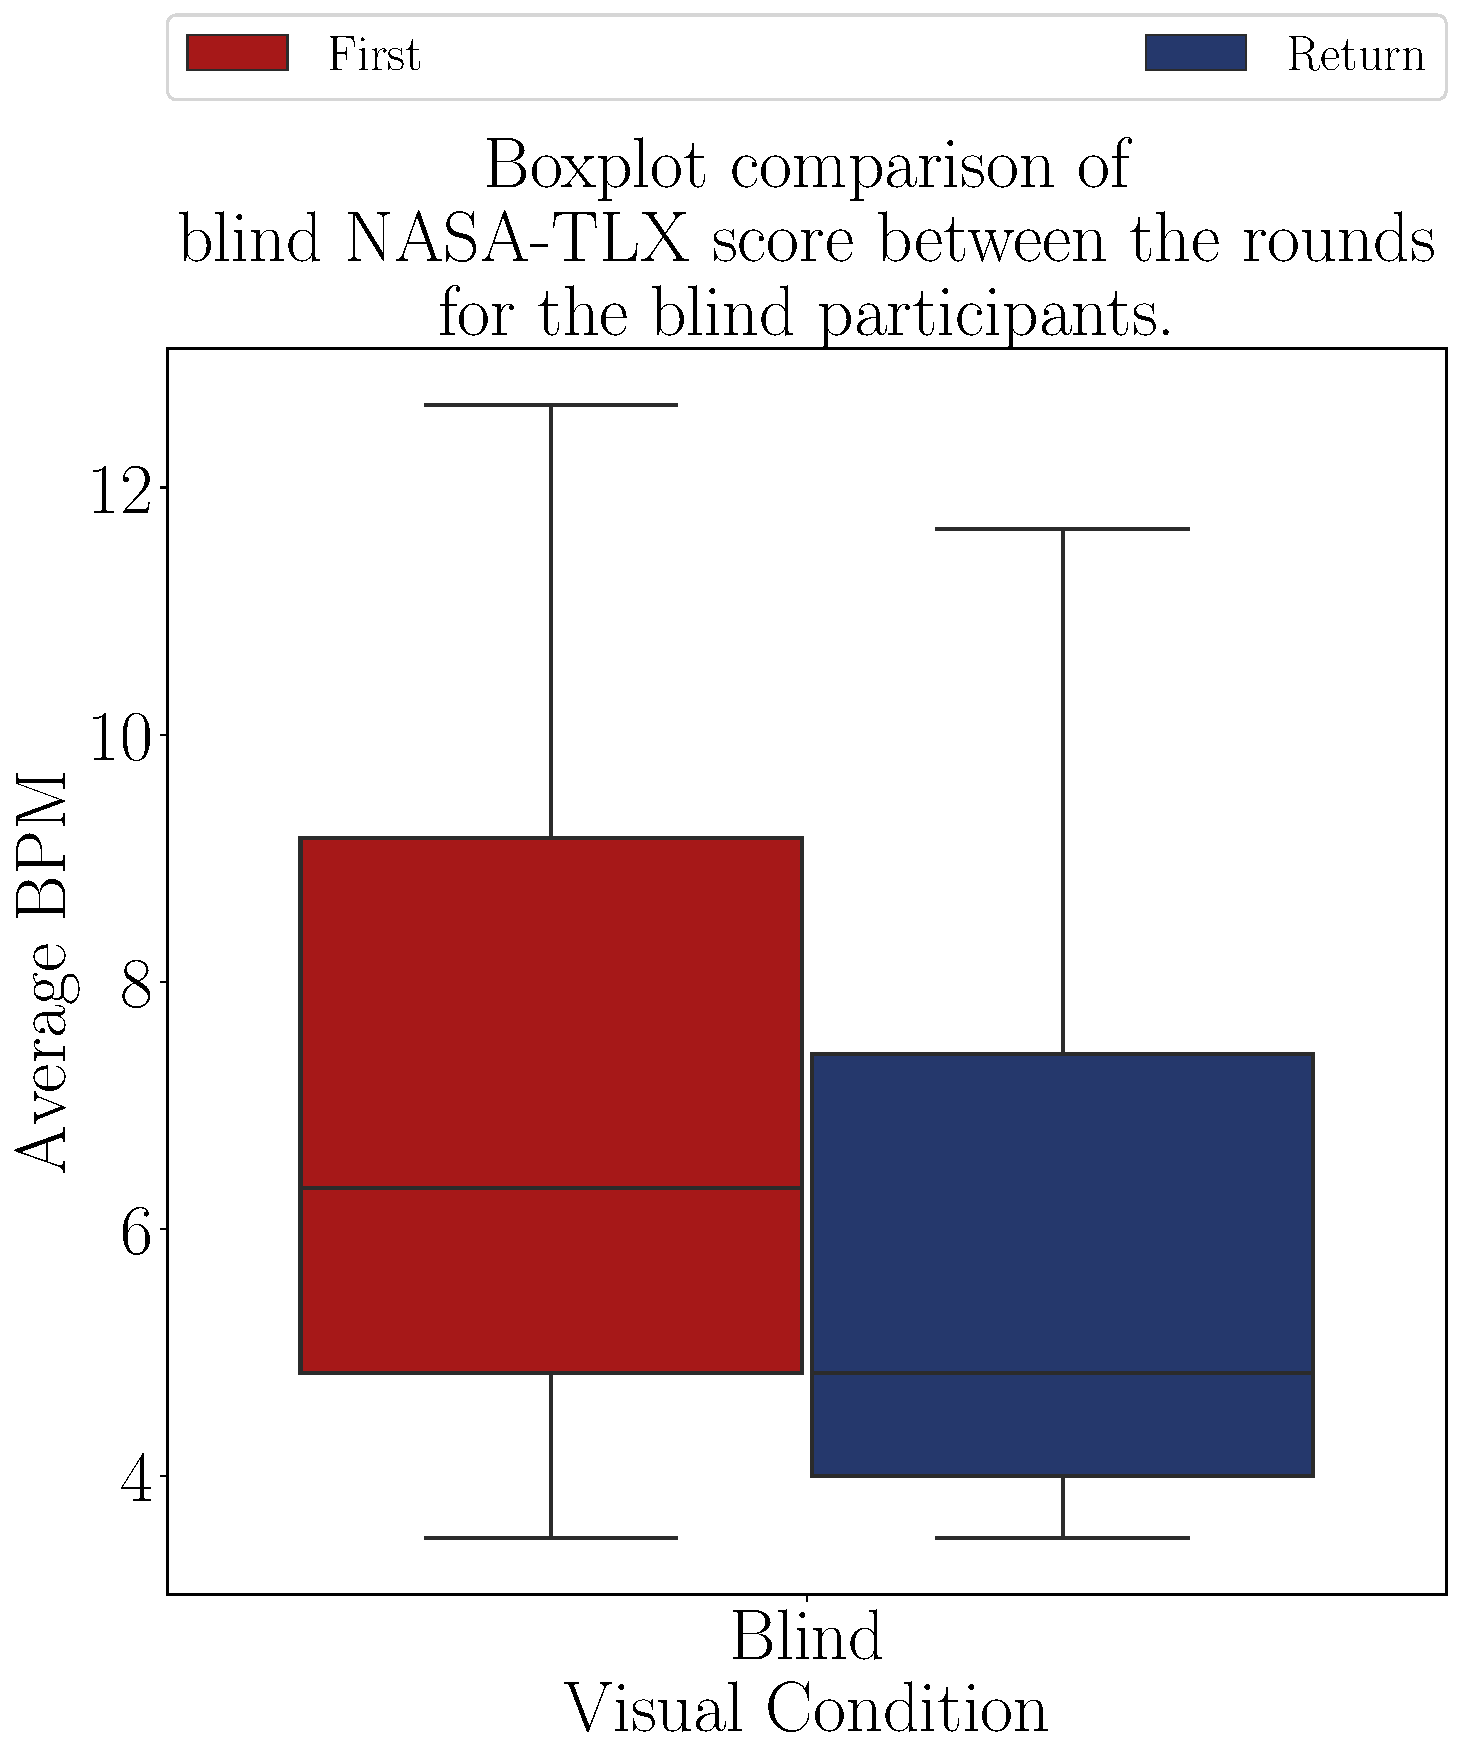
\includegraphics[width = \textwidth]{Resultados/Nasa/Figuras/pdf/boxplot_nasa_blind_rounds.pdf}
        \caption{Residual plot of the NASA-TLX score the blind participants on each method.}
        \label{fig:boxplot_nasa_blind_rounds}
    \end{minipage}
\end{figure}

Figures \ref{fig:qqplot_nasa_avg_two_way_blind} and \ref{fig:residplot_nasa_avg_two_way_blind} presents the QQ plot and residual distribution of the NASA-TLX global score, showing that apparently the data are normally distributed, but the residuals are not so homogeneous as in the previous case, showing that the participants have different variability among them.

\begin{figure}[!htb]
    \centering
    \begin{minipage}{0.45\textwidth}
        \centering
        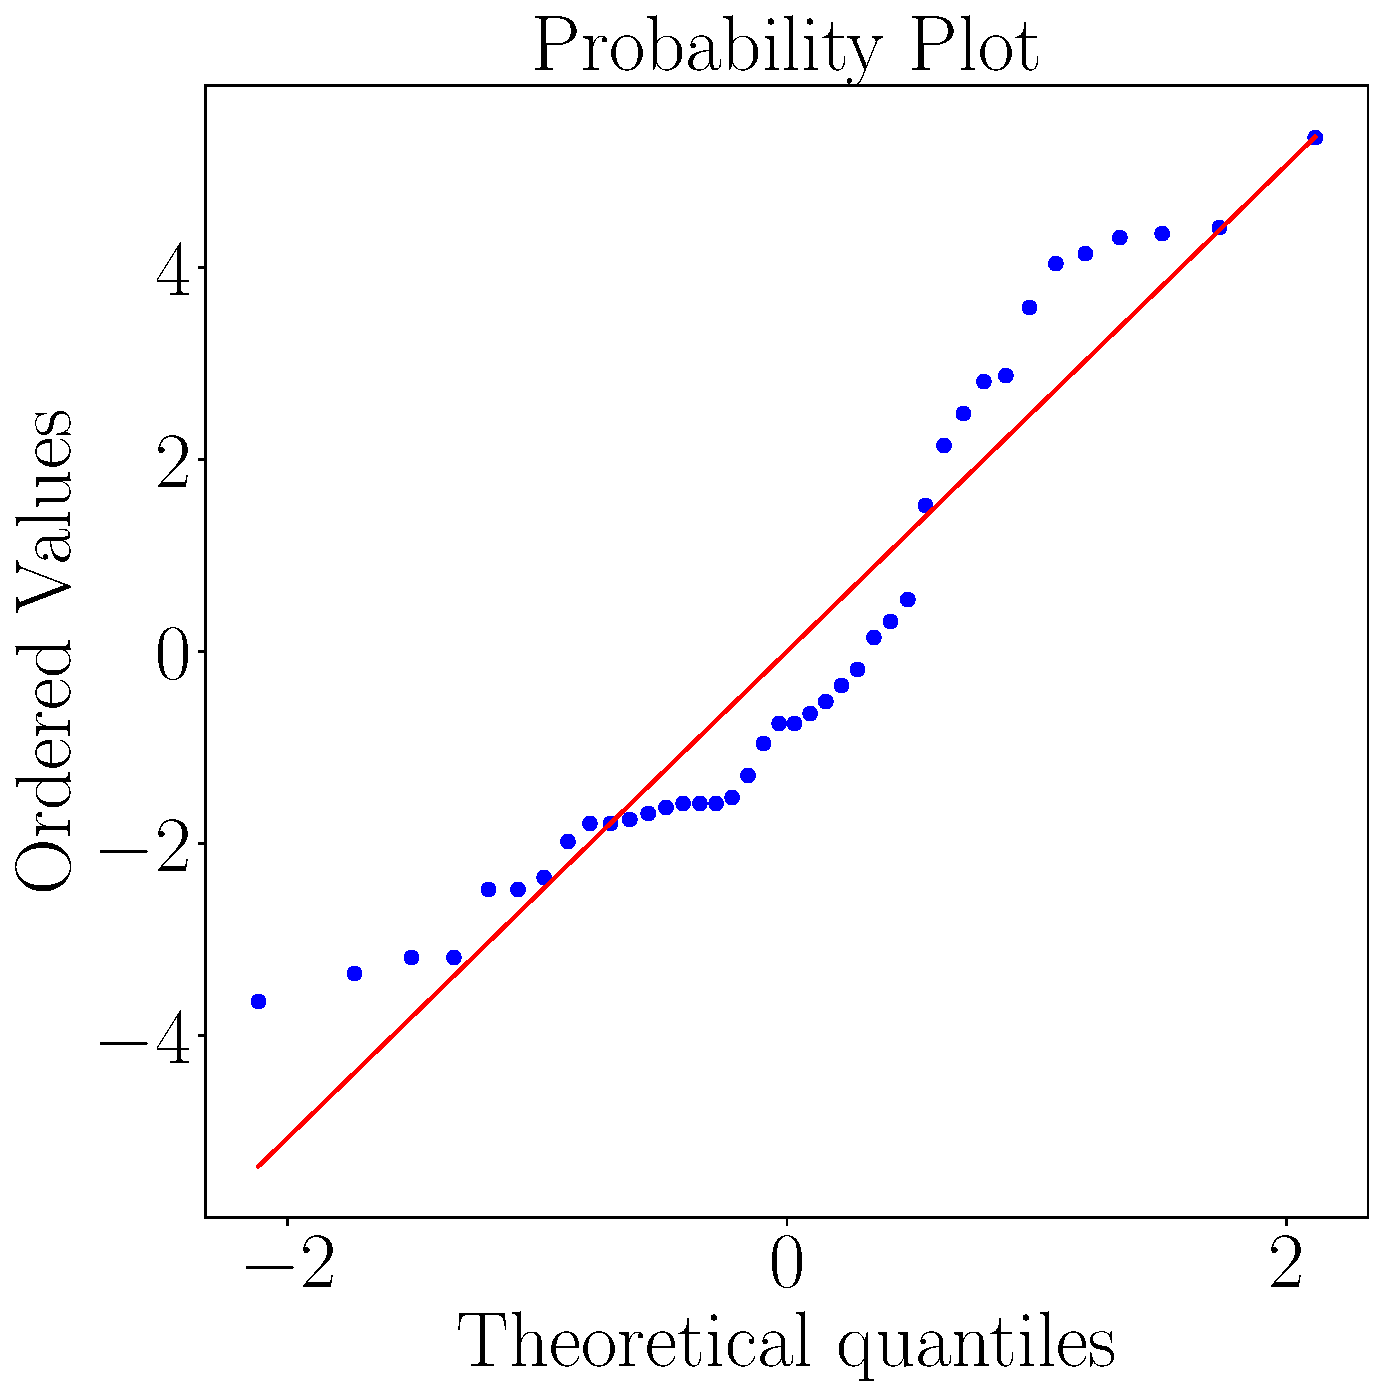
\includegraphics[width = \textwidth]{Resultados/Nasa/Figuras/pdf/qqplot_nasa_avg_two_way_blind.pdf}
        \caption{QQ plot of the NASA-TLX score variation of the blind participants on each method.}
        \label{fig:qqplot_nasa_avg_two_way_blind}
    \end{minipage}
    \begin{minipage}{0.075\textwidth}
        \hfill
    \end{minipage}
    \begin{minipage}{0.45\textwidth}
        %\vspace{2ex}
        \centering
        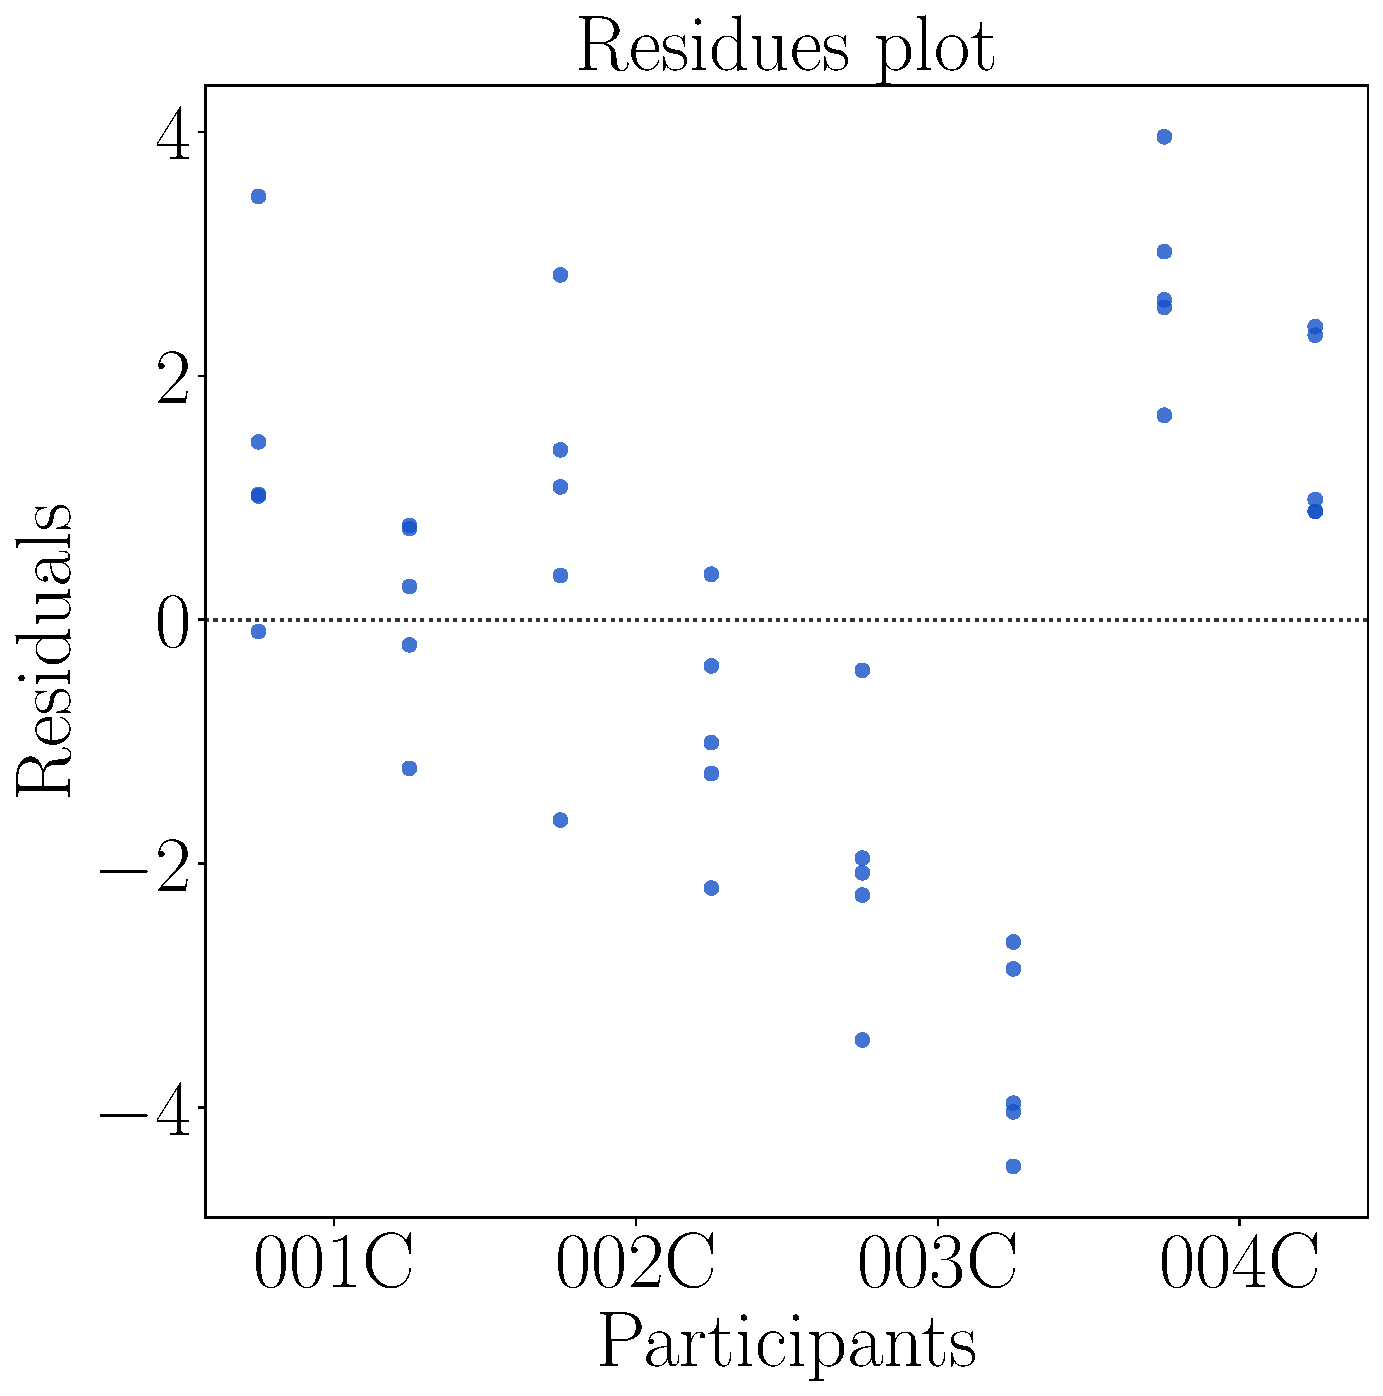
\includegraphics[width = \textwidth]{Resultados/Nasa/Figuras/pdf/residplot_nasa_avg_two_way_blind.pdf}
        \caption{Residual plot of the NASA-TLX score variation the blind participants on each method.}
        \label{fig:residplot_nasa_avg_two_way_blind}
    \end{minipage}
\end{figure}

Table \ref{tab:blocanova_nasa_avg_two_way_blind} brings the p-value resulting from ANOVA. In this case, both the method and round where appointed as significant variables that influence the mean value of the NASA-TLX global score. 


\begin{table}[!htb]
\centering
\caption{Anova p-value for the NASA-TLX score on each method for blinded users.}
\label{tab:blocanova_nasa_avg_two_way_blind}
\begin{tabular}{lrrrrl}
\toprule
          Source & P-Value \\
\midrule
    \    Methods & 0.029** \\
     \    Rounds & 0.022** \\
\    Interaction &   0.814 \\
\bottomrule
\end{tabular}
\end{table}



Finally, Table \ref{tab:lsd_nasa_avg_two_way_blind} presents the results of a pairwise Fisher LSD test comparing each pair of guidance method. The results show that only ‘audio’ is similar ‘base’, all the other methods are different among each other


\begin{table}[!htb]
\centering
\caption{Cross validation p-value for the NASA-TLX score on each method for blinded users.}
\label{tab:lsd_nasa_avg_two_way_blind}
\begin{tabular}{rclr}
\toprule
      \multicolumn{3}{c}{Method} &                                           Analysis \\
\midrule
              Base & $X$ & Audio &                   $H_0 : \mu_{Base} = \mu_{Audio}$ \\
        Base & $X$ & Haptic Belt &         $H_1 : \mu_{Base} \ne \mu_{Haptic Belt}**$ \\
       Base & $X$ & Virtual Cane &        $H_1 : \mu_{Base} \ne \mu_{Virtual Cane}**$ \\
            Base & $X$ & Mixture &             $H_1 : \mu_{Base} \ne \mu_{Mixture}**$ \\
       Audio & $X$ & Haptic Belt &        $H_1 : \mu_{Audio} \ne \mu_{Haptic Belt}**$ \\
      Audio & $X$ & Virtual Cane &       $H_1 : \mu_{Audio} \ne \mu_{Virtual Cane}**$ \\
           Audio & $X$ & Mixture &            $H_1 : \mu_{Audio} \ne \mu_{Mixture}**$ \\
Haptic Belt & $X$ & Virtual Cane & $H_1 : \mu_{Haptic Belt} \ne \mu_{Virtual Cane}**$ \\
     Haptic Belt & $X$ & Mixture &      $H_1 : \mu_{Haptic Belt} \ne \mu_{Mixture}**$ \\
    Virtual Cane & $X$ & Mixture &         $H_0 : \mu_{Virtual Cane} = \mu_{Mixture}$ \\
\bottomrule
\end{tabular}
\end{table}



Table \ref{tab:nasa_var_group_blind} shows the difference in the NASA-TLX global score between the first and return rounds. It shows that the ‘audio’ difference is the lowest among all methods, while the highest difference is for the ‘virtual cane’.


\begin{table}[!htb]
\centering
\caption{NASA-TLX score grouped by participant and visual Condition.}
\label{tab:nasa_var_group_blind}
\begin{tabular}{lrrrrrr}
\toprule
{} &   Base &  Audio & \begin{tabular}[c]{@{}l@{}}Haptic\\ Belt\end{tabular} & \begin{tabular}[c]{@{}l@{}}Virtual\\ Cane\end{tabular} & Mixture \\
Visual Condition &        &        &                                                       &                                                        &         \\
\midrule
Blind            &  -0.92 &  -0.25 &                                                 -1.21 &                                                  -1.54 &   -0.54 \\
\bottomrule
\end{tabular}
\end{table}



\FloatBarrier